\documentclass[twocolumn,a4paper]{jsarticle}

\usepackage[dvipdfmx]{graphicx}
\usepackage{amsmath}
\usepackage{mathtools}
\usepackage[top=30truemm,bottom=27mm,left=18mm,right=18mm]{geometry}

\setlength{\columnsep}{7mm}
\setlength{\abovedisplayskip}{10pt}
\setlength{\belowdisplayskip}{10pt}
\thickmuskip=1.0\thickmuskip
\medmuskip=0.8\medmuskip
\thinmuskip=0.8\thinmuskip
\arraycolsep=0.3\arraycolsep
\AtBeginDocument{
	\abovedisplayskip     =0.8\abovedisplayskip
	\abovedisplayshortskip=0.5\abovedisplayshortskip
	\belowdisplayskip     =0.8\belowdisplayskip
	\belowdisplayshortskip=0.5\belowdisplayshortskip}
\makeatletter
\renewcommand{\@cite}[1]{\textsuperscript{(#1)}}
\renewcommand{\@biblabel}[1]{(#1)}
\renewcommand{\refname}{\begin{center} 文献 \end{center} \hrulefill}
\renewcommand{\thesection}{\arabic{section}.}
\makeatother

\begin{document}
	\twocolumn[
		\centering
		\fontsize{18pt}{38mm}\selectfont
		秘密分散法の実装における速度・容量性能の評価

		\fontsize{12pt}{18mm}\selectfont
		三浦 夢生${}^{*}$,米村 恵一(木更津高専)

		\fontsize{9pt}{10mm}\selectfont
		Evaluation of speed and capacity perform in implementing secret sharing scheme

		\fontsize{9pt}{5mm}\selectfont
		Yu Miura,Keiichi Yonemura (N.I.T. Kisarazu College)
		\vspace{3mm} \\
	]

	\fontsize{9pt}{5mm}\selectfont
	\section{まえがき}
	様々なシステムやサービスがディジタル・オンライン化される流れにある現代社会において、情報の紛失や盗難への対策は重要性を増すばかりである。
	機密情報の複数人による管理や各地に配置されたサーバなどで情報の保管をする場合が例としてあげられるだろう。
	これらに対する技術として「秘密分散」があげられる。
	秘密分散とは元の秘密情報をアルゴリズムに基づいて作成した分散情報を管理する者や端末に配布・保管し、必要な数だけ集めて復元する技術のことである。この技術はクラウドサービスやブロックチェーンと相性が良いため広く用いられている。 \\
	 この技術の代表例としてShamirの提案した$(k,n)$しきい値秘密分散法\cite{shamir}があげられる。
	これは元の秘密情報から$n$個のシェアを生成し、$k$個のシェアから秘密情報の復元ができるが、$k-1$以下の個数のシェアからは元の情報は全く得られない手法である。
	本研究では、加法的秘密分散法\cite{oohara}・$(k,n)$しきい値秘密分散法\cite{shamir}・$(k,L,n)しきい値秘密分散法$\cite{yamamoto}\cite{multiparty}を実装し、実行速度及び生成されたシェアの容量について評価する。

	\section{秘密分散法}
	\subsection{加法的秘密分散法\cite{oohara}}
	加法的秘密分散法は$n$個のシェアに対して$n$個のシェアからのみ元の情報が復元できるため、$(n,n)$しきい値秘密分散法ともいえる。
	この手法はまず乱数を生成し、シェア$s_{2}=r_{1},s_{3}=r_{2},{\cdots},s_{n}=r_{n-1}$とする。
	次に秘密情報$S$を用いて以下のようにシェア$s_{1}$を生成する。
	\begin{equation}
		s_{1}=S-(s_{2}+s_{3}+{\cdots}+s_{n})
	\end{equation}
	復元の際には、参加者に配布したシェアを全て集めて足し合わせることで秘密情報$S$を得る。

	\subsection{$(k,n)$しきい値秘密分散法\cite{shamir}}
	Shamirによる$(k,n)$しきい値秘密分散法は$n$個のシェアに対して$k$個のシェアから元の秘密情報が復元できるが、$(k-1)$個以下のシェアからは元の秘密情報に関する情報は全く得られない。
	この手法は秘密情報$S$を定数項とする、ランダムな$k-1$次多項式を生成する。
	\begin{equation}
		f(x)=S+a_{1}x+a_{2}x^{2}+{\cdots}+a_{k-1}x^{k-1}
	\end{equation}
	また参加者に番号$i$を割り振り、$f(i)$を計算し、シェアとして参加者に渡す。
	復元には$k$個のシェア$(i,f(i)),i=1,2,\cdots,k$を持ち寄り、$k$個の式を立てて連立方程式を解くことで秘密情報$S$が求められる。
	このときラグランジュ補間を用いて$x=0$の場合を計算するとよい。
	\begin{align}
		L(x)={\sum_{i=0}^{k}{y_{i}l_{i}(x)}} \\
		l_{i}(x)={\prod_{j=0,j{\neq}i}^{k}{\frac{x-x_{j}}{x_{i}-x_{j}}}}
	\end{align}
	$k-1$個以下のシェアからは$k$個の式は立たず、解が求まらないため元の秘密情報に関する情報が得られないことは容易にわかる。
	コンピュータ上で連続値は扱えず、またラグランジュ補間において除算を用いているため以上の計算を有限体上で行うと都合がよい。

	\subsection{$(k,L,n)$しきい値秘密分散法\cite{yamamoto}\cite{multiparty}}
	Shamirの$(k,n)$しきい値秘密分散法を拡張した$(k,L,n)しきい値秘密分散法$は$n$個のシェアに対して$k$個のシェアから元の秘密情報が得られる。
	$k-L$個以下のシェアからは元の情報に関する情報は得られず$(k,n)$しきい値秘密分散法と比べて各シェアのサイズが$1/L$になる利点をもつが、$k-l(0{\leq}l{\leq}L-1)$個のシェアからは断片的に元の秘密情報に関する情報が得られてしまう。
	しかし、各シェアのサイズが$1/L$になる性質は非常に強力であり、実用性に長けているといえる。
	この手法は秘密情報$S$を$L$個に分割し、多項式の係数として用いる。
	\begin{equation}
		S=s_{1}||s_{2}||{\cdots}||s_{L}
	\end{equation}
	また$L$から$k-1$次の項には乱数を係数として用いて以下の多項式を生成する。
	\begin{equation}
		\begin{split}
			f(x)&=s_{1}+s_{2}x+{\cdots}+s_{L}x^{L-1} \\
			&+a_{0}x^{L}+a_{1}x^{L+2}+{\cdots}+a_{k-L-1}x^{k-1}
		\end{split}
	\end{equation}
	参加者に番号$i$を割り振り、$f(i)$を計算し、シェアとして参加者に渡す。
	復元も$(k,n)$しきい値秘密分散法と同様に連立方程式を解くことで秘密情報の断片を得た後、分割した際と逆の手順で結合を行い、元の秘密情報を得る。
	この手法における計算も有限体上で構成することでコンピュータによる実行が可能となる。

	\section{実装}
	今回はPython3.7.9及びzsh5.8においてソースコードの作成を行った。作成したプログラムの流れを図1に示す。
	秘密情報として「This is the Secret!」という文章を1万行並べた200KBのファイルを用意し、秘密分散に用いた。
	\subsection{シェルスクリプト部}
	シェルスクリプトにおいてはテキストファイルを16進数の文字列に変換し、Pythonのプログラムに渡す。
	その後、Pythonのプログラムによって生成された16進数のファイルをテキストに変換し、元のテキストファイルと再構築された秘密ファイルの差分を比較する。
	\subsection{Python部}
	ファイル入出力や秘密情報の分割については秘密分散と切り離すため別のプログラムを作成し、それぞれのアルゴリズムにインポートして使用している。
	各秘密分散には16進数を4文字ずつ読み込み、一つの10進数の秘密情報として渡している。 \\
	 加法的秘密分散法については生成するシェア数を$n=11$とし、用いる乱数の範囲を$-(2^{16}-1){\leq}r{\leq}2^{16}-1$とした。
	$(k,n)$しきい値秘密分散法ではパラメータを$k=4,n=11$に設定、有限体の標数は$p=65537$とし、復元にはラグランジュ補間を用いた。
	$(k,L,n)$しきい値秘密分散法ではパラメータを$k=4,L=2,n=11$に設定、有限体の標数は$p=65537$とし、復元にはヴァンデルモンド行列による逆行列計算を用いた。

	\begin{figure}[ht]
		\centering
		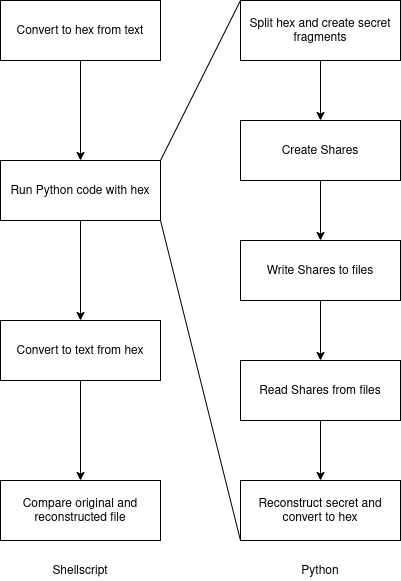
\includegraphics[keepaspectratio,scale=0.37]{program.png}
		\caption{
			\centering
			実装したプログラムの流れ \protect \linebreak
			Fig.1 Flow of the implemented program
			}
	\end{figure}

	\section{結果・考察}
	Pythonのみの実行時間を計測した結果と平均シェアサイズを表1に示す。
	加法的秘密分散法はシェアを$-(2^{16}-1){\leq}r{\leq}2^{16}-1$の範囲で生成しているため、演算を有限体上で行う他の二つと比べて平均シェアサイズが大きくなっている。
	$(k,L,n)$しきい値秘密分散法は、今回秘密情報の断片を取り出すのに逆行列計算を用いているため非常に時間がかかった結果となった。
	またシェアのサイズが$(k,n)$しきい値秘密分散法とほぼ同等であるが、これは元の秘密ファイルを一度断片に分割し、それぞれで秘密分散にかけたからだと考える。
	一つの秘密情報の断片は64ビットで分割され、どのアルゴリズムにも同様に処理されるため、今回の比較手法およびパラメータでは効果が見えなかったと考えられる。
	\begin{table}[ht]
		\centering
		\caption{
			\centering
			実行時間及びシェアの平均サイズ \protect \linebreak
			Table.1 Run time and average size of Share
			}
		\begin{tabular}{|c|c|c|c|} \hline
			アルゴリズム & 実行時間[s] & 平均サイズ[KB] \\ \hline
			\begin{tabular}{c}
				加法的 \\
				秘密分散法 
			\end{tabular}
			& 3.154 & 約637 \\ \hline
			\begin{tabular}{c}
				$(k,n)$しきい値 \\
				秘密分散法
			\end{tabular}
			& 6.956 & 約583 \\ \hline
			\begin{tabular}{c}
				$(k,L,n)$しきい値 \\
				秘密分散法
			\end{tabular}
			& 2145.62 & 約583 \\ \hline
		\end{tabular}
	\end{table}

	\section{まとめ}
	本研究では、加法的秘密分散法・$(k,n)$しきい値秘密分散法・$(k,L,n)$しきい値秘密分散法を実装し、実行速度及び生成されたシェアの容量について評価した。
	本研究の実装手法・評価項目においては$(k,n)$しきい値秘密分散法が最も優れているという結果となった。 \\
	 今後の展望として、まず$(k,L,n)$しきい値秘密分散法に適した秘密情報の断片作成方法及び秘密情報を取り出すアルゴリズムの模索をし、より適切な評価を行うことが大きな課題の一つといえる。
	次に、比較対象・評価項目を増やし、様々な観点から考察することも課題の一つと考える。具体的にはAONT秘密分散\cite{rivest}やKrawczykの方式\cite{krawczyk}などの実装や、シェアから得られる秘密情報の情報理論的評価が考えられる。

	\begin{thebibliography}{99}
		\fontsize{8pt}{4mm}\selectfont
		\bibitem{shamir}A Shamir:Communications of the ACM, 612〜613 (1979)
		\bibitem{oohara}大原:システム/制御/情報、71〜76 (2019)
		\bibitem{yamamoto}山本博資:電子通信学会論文誌、945〜952 (1985)
		\bibitem{multiparty}千田・五十嵐・菊池・濱田:研究報告コンピュータセキュリティ、1〜5 (2012)
		\bibitem{rivest}Ronald L. Rivest:Fast Software Encryption, 210〜218 (1997)
		\bibitem{krawczyk}Hugo Krawczyk:CRYPTO'93, 136〜146 (1994)
	\end{thebibliography}
\end{document}
